\chapter{Experimental Setup}
\label{chap:setup}

Knowledge about the components and techniques required for optimizing order placement was provided in Chapter \ref{chap:preliminaries}, and previous approaches were introduced in Chapter \ref{chap:related-work}.
The process of collecting historical event data and the construction of a limit order book was explained in Chapter \ref{chap:data}.
The data was investigated and hypotheses were stated as a guideline for a future learning process.
However, in order to apply reinforcement learning, an environment has to be developed which is flexible enough to allow investigation regarding different types of features and learning algorithms that are incorporated in an agent.
The correctness of such an environment is critical as it emulates a stock exchange and therefore determines how orders would have been transacted in the past.
If the implementation varies from the one used in exchanges, or does not cover certain edge cases, the matching of placed orders would differ significantly from the one in a production setup.

This chapter aims to build an environment that emulates a subset of the capabilities of a real world exchange in order to determine how limit orders would have been processed, had they been placed at a given point in time in the past.
Therefore, the setup of the environment is described at first and explains how the required components work in combination such that a learner can simulate order placement.
Additionally, an extension of this environment is provided
to simulate simultaneous order placement on both sides of the book.
This process is commonly referred to as \textit{market making}.
Finally, two implementations of reinforcement learning agents are provided.
A Q-Learning agent will serve as the learner when no market variables are provided and a Deep Q-Network agent is developed to handle complex features.


\section{Order Placement Environment}
\label{sec:setup-order-placement}

The reinforcement learning environment (see Section \ref{sec:rl-environment}) that emulates order placement on historical market data is introduced in this section and enables an agent to buy or sell $V$ shares within a time horizon $H$.
Therefore, the previously described components (introduced in Chapter \ref{chap:preliminaries}) come into play.
The main idea of its working is that, the agent observes a state $s_t$ (so-called observation state) at some time $t$ and responds with an action $a_t$ that indicates at which position to place the order in the order book, relative to the current market price.
The task of the environment is then to evaluate the outcome of the placed order and report to the agent accordingly with a reward $r_{t+1}$ and the next state $s_{t+1}$.
Subsequently, the order is cancelled such that the agent can submit a new action for the remaining shares to be bought or sold.

OpenAI Gym \cite{brockman2016openai} is an open source toolkit for reinforcement learning.
The interfaces of this toolkit were used in order to follow their standards while building this environment.
The advantage of which is that any OpenAI Gym compatible agent and bench-marking tools can make use of this environment.

\subsection{Overview of components}

\begin{figure}[H]
    \centering
    \makebox[\linewidth]{
        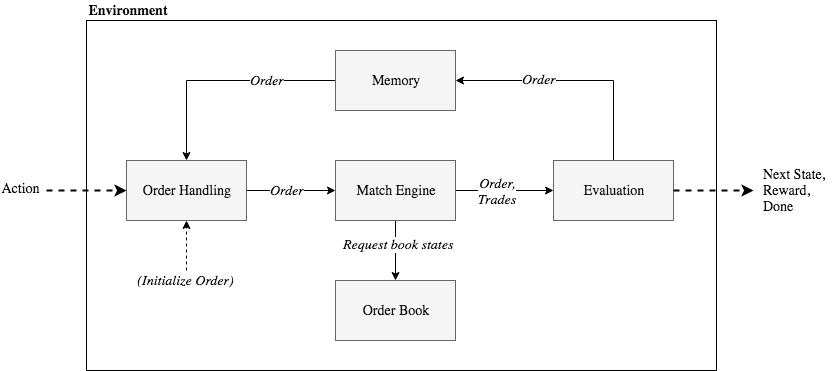
\includegraphics[width=14cm]{images/rl-env-overview}
    }
    \caption{Overview of reinforcement learning order placement environment.}
    \label{fig:rl-env-overview}
\end{figure}

Figure \ref{fig:rl-env-overview} shows the inner workings of the order placement environment.
An epoch is initialized with the \texttt{reset} function, which clears the internal state of the environment.
The internal state consists of the remaining shares the agent has to buy or sell, denoted by the \textit{inventory} $i$, the time step $t$ the agent has left to do so and the previous \textit{order}.
The agent explores the environment using the $step$ function with which it sends the action to execute.
The first component to react upon receiving the action is the \textit{order handling component}, which determines whether the agent is currently trying to fill an order, that is when the agent has started an epoch, or a new order needs to be created, that is when the agent starts an epoch.
In either case, a new order is created and the price is set according to the received action.
Subsequently, the order is forwarded to the \textit{match engine}, which tries to execute the order within the historical data set, namely the \textit{order book}.
The order and the possible resulted trades evolved during the matching process are then forwarded to the \textit{evaluation component}.
Since it can take multiple steps for the agent to fill an order, the remaining inventory and the consumed time of the order is updated and stored in the \textit{memory}.
Additionally, the index of the last visited order book state is stored such that in a next step the match engine will proceed the matching where it stopped last.
In case no trades resulted during the matching process, only the consumed time is subtracted from the order.
Otherwise, the sum of the size of the trades is subtracted from the order's inventory.
Subsequently, the evaluation component calculates the reward based on the previously resulted trades.
Finally, the reward, the next observation state and whether or not the order is completely filled (e.g. the epoch is done) is finally forwarded to the agent.
Additionally, if the order is not completely filled after the last step taken by the agent, a market order follows in order to get to the final state.

\subsection{Configuration parameters}
For the environment to be flexible, such that agents can place orders in various settings, a total of four configuration parameter have to be defined: \textit{order side (OS), time horizon (H), time step length ($\Delta{t}$)} and \textit{feature type (F)}.
The \textit{order side} $OS$ (previously defined in Eq. \ref{eq:order-side}) specifies whether the orders, which are created within the environment, are intended to be buy or sell orders.
\begin{figure}[H]
    \centering
    \makebox[\linewidth]{
        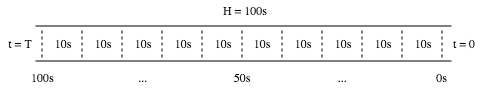
\includegraphics[width=10cm]{images/setup-time-horizon}
    }
    \caption{Segmented time horizon $H$ with remaining time $t$.}
    \label{fig:setup-time-horizon}
\end{figure}
The time horizon $H$ defines the amount of time given in order fill an order.
The default time horizon is 100 seconds for reasons described in Section \ref{sec:execution-placement}, which reflects the Good-Till-Time (see \ref{sec:ob-characteristics}) of the order.
As illustrated in Figure \ref{fig:setup-time-horizon}, the time horizon is segmented into discrete time steps $t$ and therefore limits the number of steps an agent can take within one epoch.
Each step is of the same length $\Delta{t}$, which is for illustration purposes set to 10 seconds.
We pick $T$ as the maximum value of $t$, indicating that the entire amount of time is remaining, whereas $t=0$ states that the time horizon is consumed.
Consequently, within a single epoch, the GTT of the order is being adjusted to $\Delta{t}$ for each step, still resulting in a total GTT of $H$.
Lastly, the \textit{feature type } $F$ determines the state observed by the agent, which represents one of the features described in Section \ref{sec:feature-engineering}.

\subsection{State}
\label{setup:state}
Unlike in most traditional reinforcement learning environments, each step taken by the agent leads to a complete change of the state space.
Consider a chess board environment, where the state space is the board equipped with figures. 
After every move taken by the agent, the state space would look exactly the same, except of the figures moved with that step.
The epoch would continue until the agent either wins or looses the game and the state space would be reset to the very same setup for each epoch.
In the order placement environment however, it is, as if, for each step not only one or two figures of the chess board change their position, but almost all of them.
And a reset of the environment will result in an ever changing setup of the figures on the chessboard.
The reason for this is that the chessboard is in our case the order book that underlies a time series which evolves over time.
More precisely, the state space $S$ is defined as a sequence of order book states from which an agent can observe an observation state $O$ at some point in time.
The final state is reached when the entire inventory was bought or sold, that is $i=0$--Checkmate!.
\\
\\
There are two general types of variables that can be used in order to create an observation state: \textit{private variables} and \textit{market variables} \cite{nevmyvaka2006reinforcement}.
For private variables, the size of the state space depends on the $V$ shares that have to be bought or sold and the given time horizon $H$, resulting in a state $s \in R^2$.
Market variables can be any information derived from the order book at a given moment in time.
Therefore the specified feature set (see Section \ref{sec:feature-engineering} below) defines the dimension of the state the agent observes.
Consequently, market variables increase the state space drastically, due to (1) the initialization of the environment using a random order book state and (2) the dimensionality of the feature set.
Hence, for each step taken by the agent, the order book states are likely to be different and thus the state the agent observes changes equally. 

\subsection{Action}

A discrete action space $A$ is a vector $(a_{min}, . . . , a_{max})$ that represents a range of relative limit levels an agent can choose from in order to place an order. 
That is, how deep ($a_{min}$) and how high ($a_{max}$) the order can be placed in the book.
The action $a \in A$ is an offset relative to the market price $p_{m^T}$ before the order was placed (at time step $t=T$).
Negative limit levels indicate the listing deep in the book and positive listings relate to the level in the opposing side of the book.
Hence, the price of the order placement $p$ at some time step $t$ is $p_t = p_{m^T} + a_i * \Delta{a}$, whereas $\Delta{a}$ is the step size of an action.
An illustration of this concept is given in Figure \ref{fig:setup-actions}.
\begin{figure}[H]
    \centering
    \makebox[\linewidth]{
        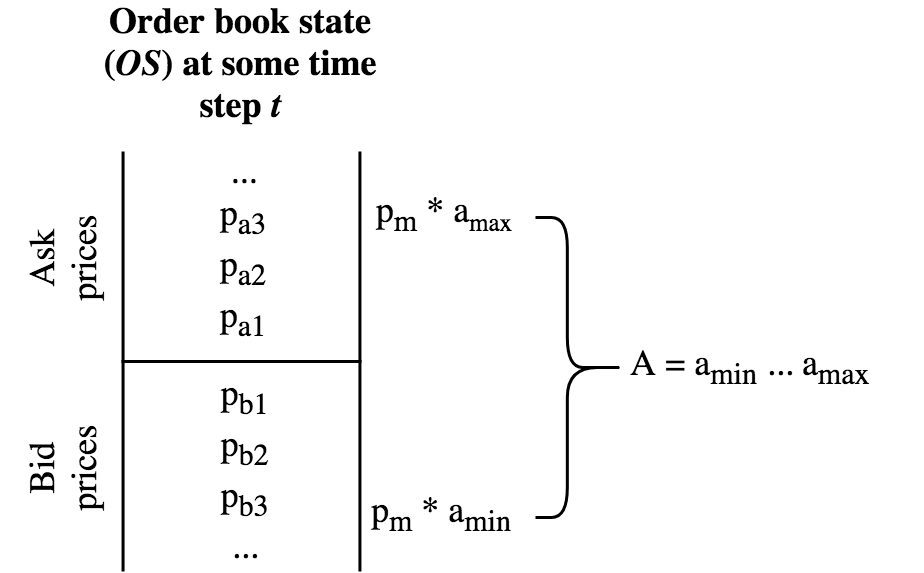
\includegraphics[width=8cm]{images/setup-actions}
    }
    \caption{Actions represent an offset relative to the order price at which to place the order in some order book state $OS_i$ at some time step $t$.}
    \label{fig:setup-actions}
\end{figure}

By default the action step size $\Delta{a}=\$0.10$.
For example, with $|A|=5$ that is $(p_{m^T}-0.2, p_{m^T}-0.1, p_{m^T}, p_{m^T}+0.1, p_{m^T}+0.2)$.
The action space is configurable and the default implementation is of size $|A|=101$, indicating that $a_{min}=-50$ and $a_{max=50}$ result in an order price $p=p_{m^T}-\$5$ and $p=p_{m^T}+\$5$ respectively.

\subsection{Reward}
\label{setup:reward}
As described in Section \ref{sec:execution-placement}, the volume weighted average price (see Eq. \ref{eq:vwap} serves as a measure of the \textit{return} of order placement.
Consequently, the \textit{reward} is defined as the difference of the market price before the order was placed $p_{m^T}$ and the volume weighted average price paid or received after the order has been filled. 
Hence, for buying assets the reward is defined as $r=p_{m^T}-p_{vwap}$ and for selling assets $r=p_{vwap}-p_{m^T}$.
In case no trades resulted during the matching process, the reward is $r=0$, indicating that no direct negative reward is provided.
Reasons for this are that in case the order could not be matched over the course of the time horizon, when $t=0$, a market order follows which will likely produces trades with a worse price than the market price before the placement has started.
Given the definition of the discounted return (Eq. \ref{eq:discounted-return}) we calculate $R_t=\sum_{t'=t}^{t_0}{\gamma^{t'-t}*r_{t'}}$, where $t_0$ is the time step at which the agent has its time horizon for the ongoing order fully consumed.

\section{Market making Environment}
TODO


\section{Q-Learning agent}
\label{setup:q-learning}

The agent described in this section is generally known as \textit{Q-Learning}\cite{watkins1992q}.
In this work, Q-Learning serves to (1) optimize order placement by using private variables only and (2) to have a measure of comparison while evaluating possible advantages of featuring raw market data by using a Deep Q-Network agent (see Section \ref{setup:dqn} below), which is an extension of the Q-Learning agent.
%However, due to the limitations of Q-Learning, which are described below, this agent cannot make direct use of the features derived in Chapter \ref{chap:data}.
%Therefore, this Section first describes the observation state that is being used by the Q-Learning agent.
%Subsequently, the Q-Learning algorithm is introduced including its use of the Bellman equation.
\\
\\
The name Q-Learning refers to the application of the previously presented Q-function (Eq. \ref{eq:q-function}).
More specifically, it relies on the \textit{action-value function} (Eq. \ref{eq:optimal-action-value-function}) that obeys an important identity known as the \textit{Bellman equation}.
The intuition is that: if the optimal value action-value $Q^*(s',a')$ of the state $s'$ at the next time step $t+1$ was known for all possible actions $a'$, the optimal strategy is to select the action $a'$ which maximizes the expected value of $r+\gamma*Q^*(s',a')$,

\begin{equation}\label{eq:bellman}
Q^*(s,a)=\mathbb{E}[r+\gamma \max_{a'} Q^*(s',a')] \ \forall{s}\in{s},  a\in{A}
\end{equation}
, whereas $0 \le \gamma \le 1$ is the discount rate which determines how mach future rewards are worth, compared to the value of immediate rewards.
The aim of the iterative value approach is to estimate the action-value function by using the Bellman equation as an iterative update,
\begin{equation}
Q_{i+1}(s,a)=\mathbb{E}[r+\gamma \max_{a'}Q_{i}(s',a')]
\end{equation}
Value iteration algorithms then converge to the \textit{optimal action-value} function $Q_{i} \rightarrow Q^*$ as $i \rightarrow \infty$. \cite{sutton1998reinforcement}
\\
\\
Q-Learning makes use of the aforementioned Bellman equation (Eq. \ref{eq:bellman}) that undergoes an iterative update.
The algorithm has proven to be an efficient and effective choice to solve problems in a discrete state space.
Limitations of this approach are known when the agent is applied to large or continuous state spaces \cite{gaskett2002q}.
This becomes more apparent when considering the presented algorithm above.
The iterative update of the action-value function $Q(s,a)$ (defined in Eq. \ref{eq:optimal-action-value-function} and used in Eq. \ref{eq:bellman}) is exposed to the size of the state $s$ and action $a$, and thus if $s$ is chosen too large, the optimal policy $\pi^*(s)$ (defined in Eq. \ref{eq:optimal-policy-s}) will likely not converge.
As a result, the features derived in Chapter \ref{chap:data} are not applicable for this agent.

However, private variables of the environment, as described in Section \ref{setup:state}, respect the aforementioned limitations.
As a result, the observation the Q-Learning agent will receive from the environment is defined by the discrete inventory unit $i$ and time step $t$, that is, $s=(i, t)$.

\begin{figure}[H]
    \centering
    \makebox[\linewidth]{
        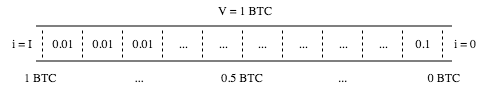
\includegraphics[width=10cm]{images/setup-inventory}
    }
    \caption{Inventory of $V$ segmented shares with a remaining inventory $i$.}
    \label{fig:setup-inventory}
\end{figure}

However, fractions of shares and time which evolve during the matching process would result in a vastly large state space.
Therefore, similar to the discrete time steps which are described above, the $V$ shares are divided into discrete inventory units $i$ of size $\Delta{i}$, as illustrated in Figure \ref{fig:setup-inventory}.
The inventory units approximate the order size in order for our policy to distinguish between when creating an order.
We pick $I$ as the maximum value of $i$, indicating that the entire inventory remains to be filled.
The order is considered as filled when $i=0$, meaning that no inventory is left.
Given the inventory units and the time steps, the state space remains $s \in R^2$ but becomes much smaller in its size, namely $I \times H$.
In the default setup a segmentation of 0.01 BTC steps is applied.
For example, if the initial inventory is 1.0 BTC and the order is partially filled with 0.015 BTC during an epoch, the remaining inventory is 0.99 BTC (instead of 0.985) for the next step the agent will take.

\begin{algorithm}
\caption{Q-Learning algorithm}\label{alg:q-learning}
\begin{algorithmic}[1]
\State Initialize $Q(s,a)$ arbitrarily
\For{each episode}
\For{t=0...T}
\For{i=0...I}
\State $s=(i, t)$
\State Choose $a$ from $s$ using $\pi$ derived from $Q$ ($\epsilon$-greedy)
\State Take action $a$, observe $r, s'$
\State $Q(s,a) \gets Q(s,a)+ \alpha[r+ \gamma \max_{a'}Q(s',a')-Q(s,a)]$
\State $s \gets s'$
\EndFor
\EndFor
\EndFor
\end{algorithmic}
\end{algorithm}
Finall, Algorithm \ref{alg:q-learning} describes the Q-Learning algorithm used in this work.
An adaption was made to a conventional Q-Learning algorithm\cite{sutton1998reinforcement} regarding the steps the agents will proceed, and therefore follows the same concept as presented in \cite{nevmyvaka2006reinforcement}.
The agent solves the order placement problem inductively, starting off the episode at state $s=(i,0)$, when $t=0$.
This has the benefit that the environment enforces a market order (see Section \ref{setup:reward}) at the beginning of an epoch, for all inventory units $i$ and therefore provides immediate reward to the agent.
The agent then increments $i$ and $t$ independently and the previously seen reward will serve as the future reward as the agent increases $i$ and $t$.
As a result, for each epoch, the agent takes $I*T$ steps.

Apart from that, the algorithm follows the standard procedure.
The Q function is updated given the state $s$ and action $a$.
Therefore, the existent estimate of the action-value function is subtracted from the value of the action that is estimated to return the maximum future reward.
In addition, a learning rate $\alpha$ is introduced that states to which extent new information should override previously learned information, with weighting $0 \le \alpha \le 1$.
Eventually, the agent completes the episode and at this point, every combination of $t$ and $i$ has been visited by the agent.
Hence, the agent has learned each discrete step $i$ and $t$ in the process of buying or selling $V$ within the time horizon $H$.

\section{Deep Q-Network agent}
\label{setup:dqn}
The second agent, which is presented in this section, is known as Deep Q-Network (mnih2015human) \cite{mnih2015human}.
DQN is a deep reinforcement learning method that combines reinforcement learning with a class
of artificial neural network known as deep neural networks.

\todo[inline]{describe NN}
%Notably, recent advances in deep neural networks9–11, in which several layers of
%nodes are used to build up progressively more abstract representations of the data, have made it possible for artificial neural networks to learn concepts such as object categories directly from raw sensory data.
%We use one particularly successful architecture, the deep convolutional network17, which uses hierarchical layers of tiled convolutional filters to mimic the effects of receptive fields--thereby exploiting the correlations present in trading activity.

Similar to the Q-Learning approach described above, the Q-values should obey the Bellman equation \ref{eq:bellman}.
The neural network treats the right-hand side, with weights $\omega$, as a target, that is, $r+\gamma \max_{a'} Q^*(s',a', \omega)$.
We then minimize the mean squared error (MSE) by stochastic gradient descent,
\begin{equation}
    L=(r+\gamma \max_{a'} Q^*(s',a', \omega') - Q(s,a,\omega))^2
\end{equation}
Whereas the optimal q-value converges for the Q-Learning approach that uses a look-up table, the use of a non-linear function approximator can cause the convergence due to (1) correlation between samples and (2) non-stationary targets.

In order to remove correlations we use \textit{experience replay} with which we build a data set $D$ from the agent's own experience.
Therefore we store the agent's experience $e_t=(s_t, a_t, r_t, s_{t+1})$ at each time-step $t$ in the data set, such that $D_t = {e_1, ..., e_t}$.
During learning process, Q-learning updates on samples (or mini-batches) of these experience $(s,a,r,s') \sim U(D)$ which are drawn uniformly at random from the pool of stored samples in $D$.
Hence, we prevent the learner from developing a pattern from the sequential nature of the experiences the agent observes throughout one epoch.
In our case this might be the case during a significant rise or fall of the market price.
In addition, experience replay stores rare experiences for much longer such that the agent can learn these more often.
That is for example when massive subsequent buy order led to a noticeable change in the order book.

In order to deal with non-stationarity, the target network parameters $\delta'$ are only updated with $\delta$ every C steps and otherwise unchanged between individual updates.
